\documentclass[12pt,a4paper]{article}

\usepackage[utf8]{inputenc}
\usepackage{amsmath}
\usepackage{amsfonts}
\usepackage{amssymb}
\usepackage{graphicx}
\usepackage{placeins}
    
\usepackage[left=2.5cm,right=2.5cm,top=2cm,bottom=3cm]{geometry}
    
\usepackage[round]{natbib}
\usepackage{hyperref}

%%%%%%%%%%%%%%%% Code Listing %%%%%%%%%%%%%%%%%%%%%%%%%%%%%%%
\usepackage{listings}
\usepackage{color}

\definecolor{mygreen}{rgb}{0,0.6,0}
\definecolor{mygray}{rgb}{0.5,0.5,0.5}
\definecolor{mymauve}{rgb}{0.58,0,0.82}

\lstset{ %
  backgroundcolor=\color{white},   % choose the background color; you must add \usepackage{color} or \usepackage{xcolor}
  basicstyle=\footnotesize,        % the size of the fonts that are used for the code
  breakatwhitespace=false,         % sets if automatic breaks should only happen at whitespace
  breaklines=true,                 % sets automatic line breaking
  captionpos=b,                    % sets the caption-position to bottom
  commentstyle=\color{mygreen},    % comment style
  deletekeywords={...},            % if you want to delete keywords from the given language
  escapeinside={\%*}{*)},          % if you want to add LaTeX within your code
  extendedchars=true,              % lets you use non-ASCII characters; for 8-bits encodings only, does not work with UTF-8
  frame=single,                    % adds a frame around the code
  keepspaces=true,                 % keeps spaces in text, useful for keeping indentation of code (possibly needs columns=flexible)
  keywordstyle=\color{blue},       % keyword style
  language=Matlab,                 % the language of the code
  morekeywords={*,...},            % if you want to add more keywords to the set
  numbers=left,                    % where to put the line-numbers; possible values are (none, left, right)
  numbersep=5pt,                   % how far the line-numbers are from the code
  numberstyle=\tiny\color{mygray}, % the style that is used for the line-numbers
  rulecolor=\color{black},         % if not set, the frame-color may be changed on line-breaks within not-black text (e.g. comments (green here))
  showspaces=false,                % show spaces everywhere adding particular underscores; it overrides 'showstringspaces'
  showstringspaces=false,          % underline spaces within strings only
  showtabs=false,                  % show tabs within strings adding particular underscores
  stepnumber=2,                    % the step between two line-numbers. If it's 1, each line will be numbered
  stringstyle=\color{mymauve},     % string literal style
  tabsize=2                        % sets default tabsize to 2 spaces
}
%%%%%%%%%%%%%%%%%%%%%%%%%%%%%%%%%%%%%%%%%%%%%%%%%%%%%%%

\usepackage{textcomp}

\author{
  A. Theodorou\\
  \texttt{theoda@ipta.demokritos.gr}
  \and
  G. Apostolopoulos\\
  \texttt{gapost@ipta.demokritos.gr}
}

\date{June 2021}
\title{\texttt{pcpsim} \\ 
Precipitation Kinetics Simulation in \texttt{MATLAB/OCTAVE}
}
     
\begin{document}

\maketitle

\section{Introduction}
\texttt{pcpsim} is a collection of \texttt{MATLAB/OCTAVE} scripts that can be used to simulate homogeneous precipitation of a 2nd phase in alloys. 

The underlying model is that of \citet{Langer-1980-Kineticsofnucleati}, as modified by \citet{Kampmann-1984-KINETICSOFPRECIPIT} (MLS model) and describes the nucleation and growth of  precipitates from a supersaturated solid solution.


\section{Theoretical background}

\subsection{Nucleation}

The driving force for precipitation is the free energy gain: 
\begin{equation}
\Delta g = - \frac{kT}{V_{at}} \cdot S 
\end{equation}
with
\begin{equation}
S =  X_p \ln\frac{X}{X_{eq}} + (1 - X_p) \ln\frac{1 - X}{1-X_{eq}} 
\end{equation}
where $V_{at}$ is the atomic volume of the new phase, $S$ is a thermodynamical function derived by \citet{Aaronson-1970-Thevolumefreeener}, $X_{eq}$ is the equilibrium solute mole fraction in the matrix, $X_p$ the solute mole fraction in the precipitate, and $X$ the current solute mole fraction in the matrix. 

The nucleation rate is \citep{Kampmann-1984-KINETICSOFPRECIPIT}
\begin{equation}
\label{eq:nucleation}
\frac{d N}{d t} = Z \beta^* \exp(-\frac{\Delta G^*}{kT}) \exp(-\frac{t_i}{t})
\end{equation}
where $N$ is the number of nuclei per atomic site, $Z$ is the Zeldovich factor ($\approx$ 1/20) and $t_i$ is the incubation time. The other parameters of equation are expressed as follows:
\begin{subequations}
	\begin{align}
\beta^* &= \frac{4\pi R^{*2} D X}{a^4} \\
R^* &= \frac{2\gamma V_{at}}{S\,kT} \\
\Delta G^* &= \frac{4}{3}\pi R^{*2}\gamma \\
t_i &= \frac{1}{2\beta^* Z} 
	\end{align}	
\end{subequations}
where $R^*$ and $\Delta G^*$ are the critical nucleation radius and free energy, respectively, $\gamma$ is the matrix/precipitate interfacial energy and $D$ is the diffusion coefficient of solute atoms in the matrix.


\subsection{Growth}

A spherical precipitate with $R>R^*$ grows by incorporating solute atoms from the surrounding matrix. Thus there is a flow of solute atoms from the supersaturated matrix towards the precipitate surface. It is assumed that a steady-state is reached where there is a constant gradient of the solute concentration around the precipitate $X(r)$ that supports the solute flow $J = -D\,dX/dr |_{r=R}$, where $D$ is the diffusion constant of solute atoms in the matrix.

By solving the steady-state diffusion equation $\nabla^2 X(r)=0$ in the region around the precipitate the following equation is obtained
\begin{equation}
\frac{dR}{dt} = \frac{D}{R} \; \frac{X-X_R}{X_p-X_R}
\label{eq:growth}
\end{equation}
where $X_R$ is the solute concentration at the matrix/precipitate interface.
$X_R$ should be equal to the equilibrium concentration as modified by the Gibbs-Thomson effect (surface tension). In the \textit{ideal solution} approximation $X_R$ is given by \citep{Calderon-1994-Ostwaldripeningin}:
\begin{equation}
X_R =  X_{eq} \cdot \exp \left( \frac{2\gamma V_{at}}{kT\, R} \frac{1-X_{eq}}{X_p - X_{eq}}\right) 
\end{equation}

\subsection{Coarsening}

When the system reaches the coarsening region the average precipitate radius grows as
\begin{equation}
R^3(t) = K\cdot t
\end{equation}
where $K$ is given in the \textit{ideal solution} approximation by \citep{Calderon-1994-Ostwaldripeningin}
\begin{equation}
K\approx K_{\text{IS}} = \frac{8}{9}\frac{D \gamma V_{at}}{kT}\;
\frac{X_{eq}\, (1-X_{eq})}{(X_p - X_{eq} )^2}
\end{equation}
Thus the time differential of $R$ is given by
\begin{equation}
\frac{dR}{dt} = \frac{8}{27}\;
\frac{D \gamma V_{at}}{kT\,R^2}\;
\frac{X_{eq}\, (1-X_{eq})}{(X_p - X_{eq} )^2}
\end{equation}

\section{MLS equation for the mean precipitate radius}

In the general case there is a precipitate size distribution and one has to study its evolution. However, in the MLS model we consider only the mean radius $\bar{R}$. It has been shown that in many cases this is sufficient.

In this approximation $\bar{R}$ grows according to \eqref{eq:growth} while new precipitates of radius $R^*$ nucleate at a rate given by \eqref{eq:nucleation}. The combination of these 2 processes leads to the following equation 
\begin{equation}
\label{eq:mls}
\frac{d\bar{R}}{dt} = \frac{D}{\bar{R}} \cdot \frac{X - X_R}{X_p - X_R} - \frac{1}{N}\frac{dN}{dt} \cdot (\bar{R} - \alpha R^*)
\end{equation}
where the 2nd term expresses the reduction rate of $\bar{R}$ due to the nucleation of new critical nuclei. $\alpha$ is a value just above 1 (e.g. 1.05) which reflects the fact that new precipitates grow only if their size is slightly larger than the critical size.

As precipitates grow they consume solute atoms and thus the matrix concentration $X$ will be reduced from the initial $X_0$. The solute balance can be expressed as:
\begin{equation}
\label{eq:balance}
X_0 = X\,(1-F) + X_p\,F
\end{equation}
where $F=\frac{4}{3}\pi R^3 N$ is the precipitate volume fraction.

The equations \eqref{eq:nucleation}, \eqref{eq:mls} and \eqref{eq:balance} form a differential-algebraic (DAE) system which can be integrated numerically in \texttt{MATLAB/OCTAVE}. 

\section{Dimensionless formulation}
To facilitate coding we define the following dimensionless variables:
\begin{subequations}
	\label{eq:dmls}
	\begin{align}
t' &= t / \tau \\
R' &= R / r_{at}
	\end{align}
\end{subequations}
where $r_{at} = (3V_{at}/4\pi)^{1/3}$ is the atomic radius and $\tau = r_{at}^2/D$ corresponds roughly to the time between atomic jumps.

The complete DAE system in terms of dimensionless variables becomes:
\begin{subequations}
\label{eq:ngdae}
\begin{align}
\frac{dN}{dt'} &= 
\frac{\beta_0 X}{S^2} 
\exp\left( -\frac{\Delta G_0}{S^2}\right)  
\exp\left( -\frac{S^2}{2\beta_0 X t'}\right)  \\
%%%%
\frac{dR'}{dt'} &=  
\frac{X - X_R}{X_p - X_R} 
\; \frac{1}{R'}
+ 
\frac{1}{N}\frac{dN}{dt'}
\left( \frac{\alpha R_0}{S} - R' \right) \\
X_0 &= X\,(1-F) + X_p\,F
\end{align}
\end{subequations}
where the following additional definitions were introduced
\begin{subequations}
\label{eq:ngparam}
\begin{align}
R_0 &= \frac{2\gamma V_{at}}{r_{at}kT} \\ 
\beta_0 &= 4\pi R_0^2 Z r_{at}^4/ a^4 \\
\Delta G_0 &= R_0^3/2  
\end{align}
\end{subequations}

Further, the following also hold
\begin{subequations}
\begin{align}
X_R &= X_{eq} \exp 
\left( \frac{R_0}{R'} \frac{1-X_{eq}}{X_p - X_{eq}}\right) \\
F &= R'^3 N
\end{align}
\end{subequations}

In the following we will omit the prime from $t'$ and $R'$.

\section{Implementation in \texttt{MATLAB/OCTAVE}}

The implementation is done in the following scripts:

\begin{description}
\item[\texttt{m/ng.m}] This function implements the nucleation and growth equations, i.e., the first two of \eqref{eq:ngdae}

\item[\texttt{m/ngdae.m}] This is a driver function for the solution of the DAE system. The user chooses the solver, either \texttt{ode15i} or  \texttt{daspk}. 

\item[\texttt{m/ngparam.m}] This utility function calculates all parameters of the dimensionless formulation, equations \eqref{eq:ngparam} and \eqref{eq:dmls}, given the physical model parameters in SI units.

\end{description}

Details on the use of these functions can be found in the included examples, in the project sub-folders \texttt{FeC} and \texttt{FeN}. 

\pagebreak

\section{Example calculations}

\subsection{Nucleation of Fe$_3$C carbide}

In this example we repeat a calculation reported by \citet{Perez-2003-ID509} to validate our programs.

All model parameters are taken from this publication. The results are very similar.

\begin{figure}[h]
\centering 
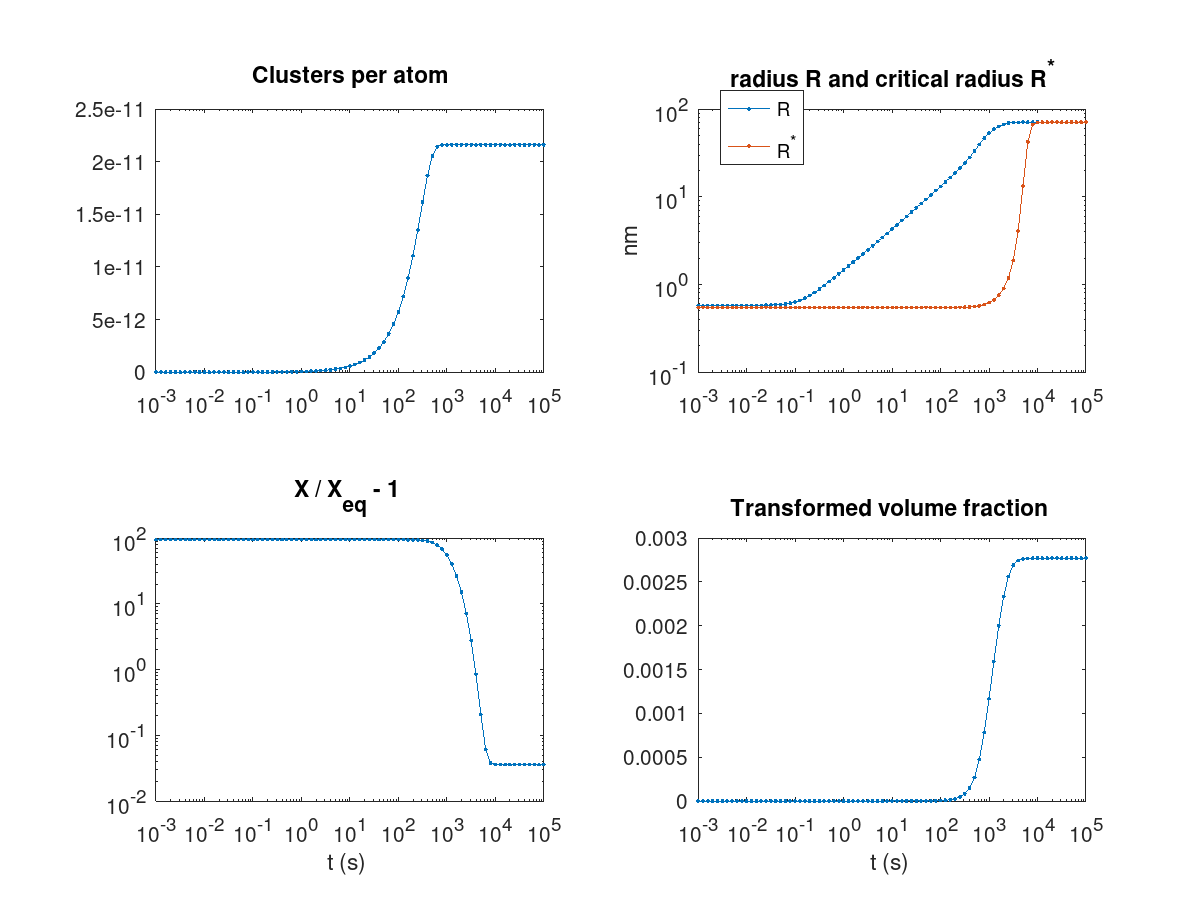
\includegraphics[width=\textwidth]{../FeC/Fe3C_nucl.png} 
\caption{\texttt{FeC/Fe3C\_nucl.m} Nucleation of Fe$_3$C carbide in a Fe - 0.07 at.\% C alloy at 487~K. Model parameter: $\gamma = 0.174$~J/m$^2$. Compare to \citet{Perez-2003-ID509}}
\end{figure}

\pagebreak

\subsection{Nucleation of $\alpha ''$ nitride at 373 K}

This calculation is very similar to the previous example and aims to simulate the precipitation of $\alpha ''$-Fe$_16$N$_2$ metastable nitride  in a Fe-N solid solution. This phase forms during low temperature ageing of Fe-N alloys (room temperature to 150$^\circ$C) and dissolves at about 250$^\circ$C \citep{Jack-1994-ID1207}.

For the diffusion of interstitial N in Fe we used the following parametrization from (A.D. Le Claire, Landolt-B{\"o}rnstein, 1990)
\begin{equation}
D(\text{m}^2/\text{s}) = 1.26\times 10^{-7}
\exp\left( -0.76\text{ eV}/k_B T \right) 
\end{equation}
and for the N concentration in the Fe matrix, in equilibrium with the $\alpha ''$ we consider
\begin{equation}
X_{eq} = 2.69
\exp\left( -0.37\text{ eV}/k_B T \right) 
\end{equation}
as reported in \citet{Wriedt-1987-ID1192}. 

For the surface energy we assume the value $\gamma = 0.06$~J/m$^2$ in order to obtain nucleation times similar to those observed in the experiments of \citet{Abiko-1977-ID656}.


\begin{figure}[h]
\centering
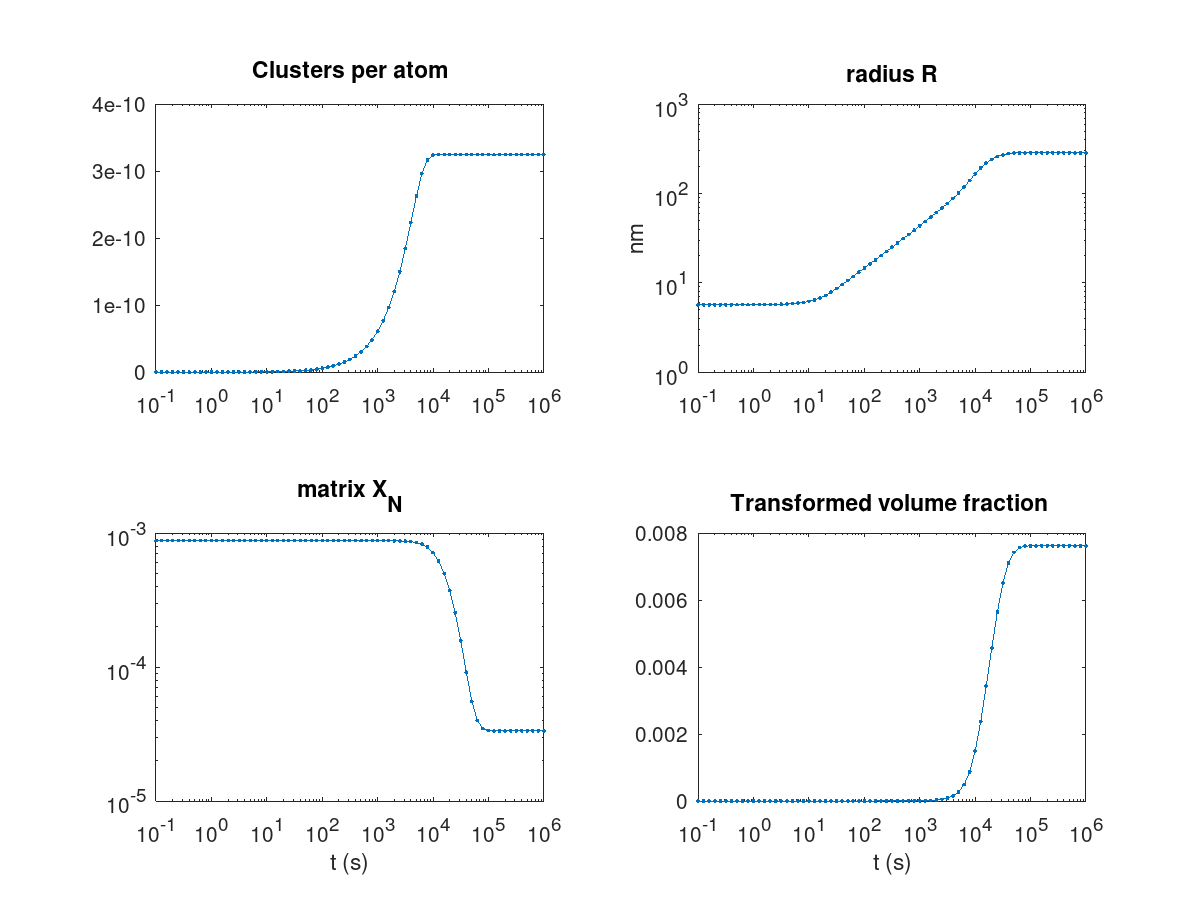
\includegraphics[width=\textwidth]{../FeN/FeN_isothermal_nucl.png} 
\caption{\texttt{FeN/FeN\_isothermal\_nucl.m} Nucleation of $\alpha ''$ nitride in a 
Fe - 0.088 at.\% N alloy at 373~K. 
Model parameter: $\gamma = 0.06$~J/m$^2$.
}
\end{figure}

\pagebreak

\subsection{Nucleation/Dissolution of $\alpha ''$ nitride during isochronal annealing}

The MLS model is actually not well suited for dynamic/transient processes like isochronal annealing where we have frequent temperature changes. 
For example, suppose some particles have nucleated at a temperature $T_1$ with radius $R\sim R_1^*$ in the course of an isochronal annealing process. When the system is brought to a higher temperature $T_2>T_1$, where $R<R_2^*$, then the particles are unstable and will dissolve. However, this cannot be properly described by the MLS equations.

Nevertheless, here we make the following approximation in order to simulate nitride nucleation/dissolution by means of the MLS model. If at some temperature during the nucleation phase the existing particles are below $R^*$, they are immediately ``dissolved'' and the nucleation process starts again from scratch. This is implemented as follows. Suppose that after some ageing process we have a concentration $N$ of nuclei with mean radius $R$. The ageing will continue at a temperature $T$. We decide if the nuclei will survive based  on the following steps:
\begin{itemize}
\item Calculate the critical radius $R^*$ at the new temperature
\item Calculate the nucleation rate $J_n$ at the new temperature
\item If $R<R^*$ and $J_n \neq 0$ set $N=0$, $X=X_0$ and $R=R^*$ (dissolve the nuclei)
\end{itemize}

This model is implemented in \texttt{FeN/FeN\_isochronal\_nucl.m} where a Fe - 0.047 at.\% N alloy is subjected to the following annealing program: $280 < T < 600$~K, $\Delta T=10$~K, $\Delta t=5$~min. During the process we observe the nucleation of $\alpha''$ at about 350~K and its subsequent dissolution above 450~K. Model parameters ($D$, $X_{eq}$, $\gamma$) are the same as in the preceding section.

The simulation results for particle radius, density, volume fraction as a function of temperature are shown in the following figure. 

\begin{figure}[b]
\centering
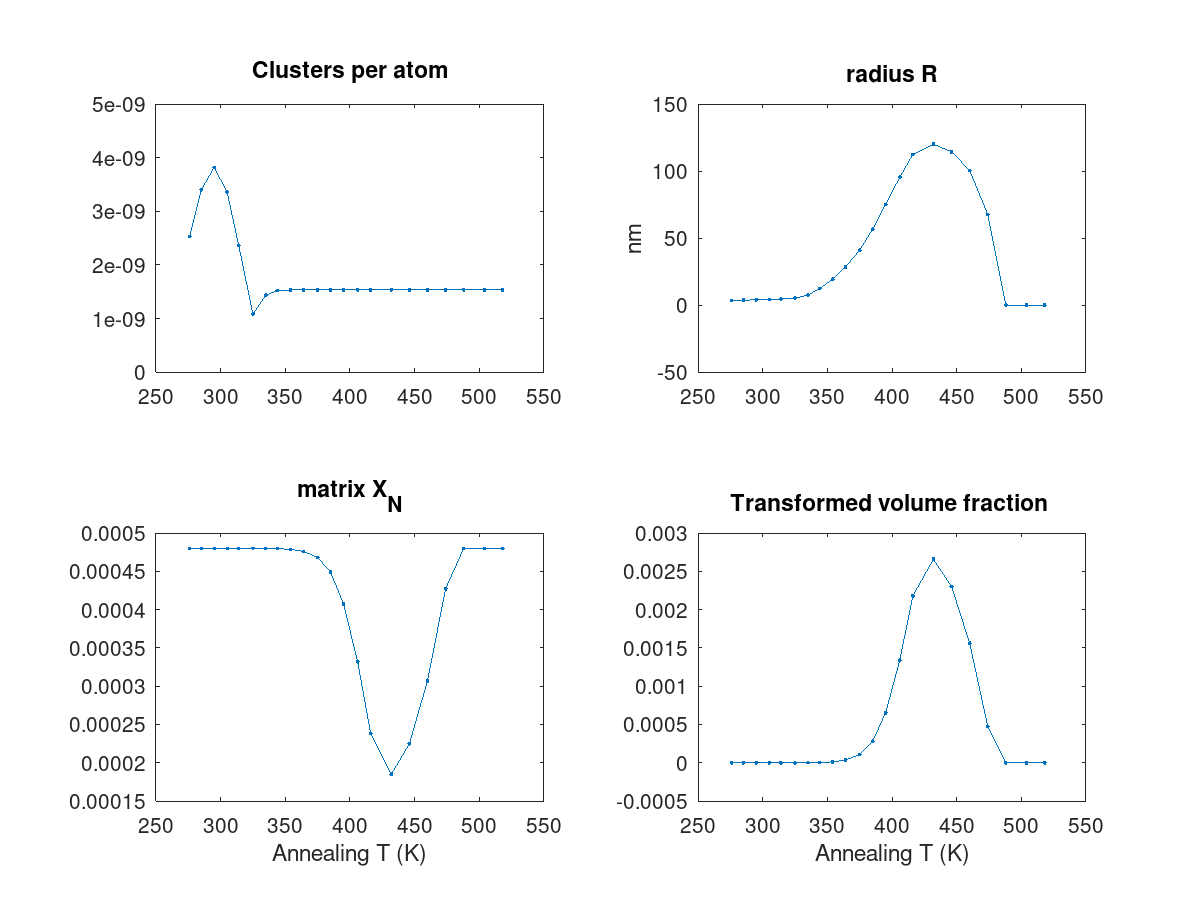
\includegraphics[width=\textwidth]{../FeN/FeN_isochronal_nucl.png} 
\caption{\texttt{FeN/FeN\_isochronal\_nucl.m} Nucleation and dissolution of $\alpha ''$ nitride in a Fe - 0.047 at.\% N alloy during isochronal annealing. Model parameter: $\gamma = 0.06$~J/m$^2$. }
\end{figure}

\pagebreak
\FloatBarrier



 
\bibliographystyle{plainnat}
\bibliography{pcpsim}
%\bibliography{/home/george/Work/Sci/Pubs/bib/export.bib}

\end{document}
 